\documentclass[tikz,border=8pt]{standalone}

% общий стиль (подключается через TEXINPUTS)
% tikz-style.tex (общий стиль для всех TikZ-картинок)
\RequirePackage[T1,T2A]{fontenc}
\RequirePackage[utf8]{inputenc}

% Palatino-подобный шрифт (как в MathJax часто воспринимается «более вытянутым»)
\RequirePackage{txfonts}
% txfonts даёт предупреждение по кириллице (T2A/txr не определён).
% Оставляем txfonts для математики, а текстовый шрифт возвращаем на Computer Modern,
% чтобы не искать T2A/txr и убрать предупреждения.
\renewcommand{\rmdefault}{cmr}
\renewcommand{\sfdefault}{cmss}
\renewcommand{\ttdefault}{cmtt}

\RequirePackage{tikz}
\RequirePackage{xcolor}
\usetikzlibrary{calc}

% цвета
\definecolor{lightgreen}{RGB}{214,234,214}
\definecolor{darkgreen}{HTML}{0B7A0B}
\definecolor{darkred}{HTML}{DF0000}

\definecolor{midgreen}{HTML}{2E9B2E}
\definecolor{palegreen}{RGB}{235,246,235}
\definecolor{olivegreen}{HTML}{3E6B2F}

\definecolor{lightred}{RGB}{255,220,220}
\definecolor{midred}{HTML}{E04545}
\definecolor{darkred2}{HTML}{A80000}

\definecolor{lightblue}{RGB}{220,232,255}
\definecolor{midblue}{HTML}{2E5BD6}
\definecolor{darkblue}{HTML}{0B2E8A}

\definecolor{lightgray}{RGB}{240,240,240}
\definecolor{midgray}{RGB}{170,170,170}
\definecolor{darkgray}{RGB}{80,80,80}

\definecolor{vtxfill}{RGB}{86,193,255}
\definecolor{vennfill}{RGB}{220,232,255}


% единый набор стилей TikZ
\tikzset{
    lab/.style={
        font=\fontsize{24}{32}\selectfont
    }
}


\usepackage{tikz}
\usetikzlibrary{arrows.meta}

\begin{document}
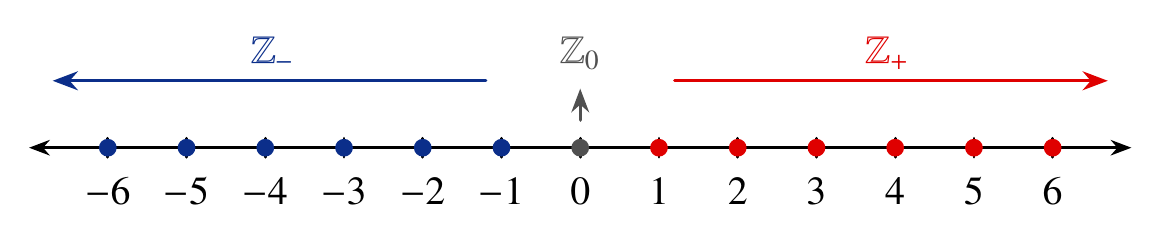
\begin{tikzpicture}[x=1cm,y=1cm,line cap=round,line join=round]

% main number line
\draw[line width=1.0pt, <->, >=Stealth] (-7,0) -- (7,0);

% integer ticks, labels, and colored points
\foreach \x in {-6,-5,...,6} {
  \draw[line width=1.0pt] (\x,0.12) -- (\x,-0.12);
  \node[font=\Large] at (\x,-0.55) {$\x$};

  \ifnum\x<0
    \fill[darkblue] (\x,0) circle (3.2pt);
  \else\ifnum\x>0
    \fill[darkred] (\x,0) circle (3.2pt);
  \else
    \fill[darkgray] (\x,0) circle (3.2pt);
  \fi\fi
}

% labels for Z-, Z0, Z+
\draw[darkblue, line width=1.2pt, -{Stealth[length=3.2mm]}] (-1.2,0.85) -- (-6.7,0.85);
\node[font=\Large, text=darkblue] at (-3.9,1.2) {$\mathbb{Z}_{-}$};

\draw[darkred, line width=1.2pt, -{Stealth[length=3.2mm]}] (1.2,0.85) -- (6.7,0.85);
\node[font=\Large, text=darkred] at (3.9,1.2) {$\mathbb{Z}_{+}$};

\draw[darkgray, line width=1.2pt, -{Stealth[length=3.0mm]}] (0,0.35) -- (0,0.75);
\node[font=\Large, text=darkgray] at (0,1.2) {$\mathbb{Z}_{0}$};

\end{tikzpicture}
\end{document}
